\begin{frame}{Variante de l'algorithme de Ford \& Fulkerson}
    \begin{itemize}
        \item L'algorithme vu en cours est efficace mais peu évident à appliquer \emph{visuellement}
        \item On peut modifier la recherche de chaine augmentante sans utiliser le graphe résiduel
        \item Principe 
        \begin{itemize}
            \item Repérer les chaines augmentantes \emph{de visu} et augmenter le flot en conséquence 
            \item Utiliser un simple algorithme de marquage pour repérer de nouvelles chaines augmentantes
        \end{itemize}
    \end{itemize}
\end{frame}

\begin{frame}{Recherche de chaine augmentante}
\begin{tabbing}
    \= xx \= xx \= xx \= xx \= xx \=
    xxxxxxxxxxxxxxxxxxxxxxxxxxxxxxxxxxxxxxxxxxxxxxxxxxx\kill
    \> Soit $x$ un flot admissible, marquer \textbf{+} le sommet $s$ \\
    \> \textbf{Répéter} \\
    \> \> \textbf{Si} $i$ est marqué et $j$ non marqué \textbf{Alors} \\
    \> \> \> \textbf{Si} $(i,j)$ est un arc non saturé \textbf{Alors} \\
    \> \> \> \> marquer $j$ avec \textbf{+} \\
    \> \> \> \textbf{FinSi} \\
    \> \> \> \textbf{Si} $(j,i)$ est un arc tel que $x_{ij} > 0$  \textbf{Alors} \\
    \> \> \> \> marquer $j$ avec \textbf{-} \\
    \> \> \> \textbf{FinSi} \\
    \> \> \textbf{FinSi} \\
    \> \textbf{Jusqu'à} ce qu'on ne puisse plus marquer de sommets \\
    \> \textbf{Si} $t$ est marqué \textbf{Alors} \\
    \> \> il existe une chaîne augmentante de $s$ à $t$ \\
    \> \> augmenter le flot et recommencer \\
    \> \textbf{Sinon} \\
    \> \> le flot est maximal \\
    \> \textbf{FinSi} \\
  \end{tabbing}

  
\end{frame}

\begin{frame}{graphe initial}
        \begin{center}
            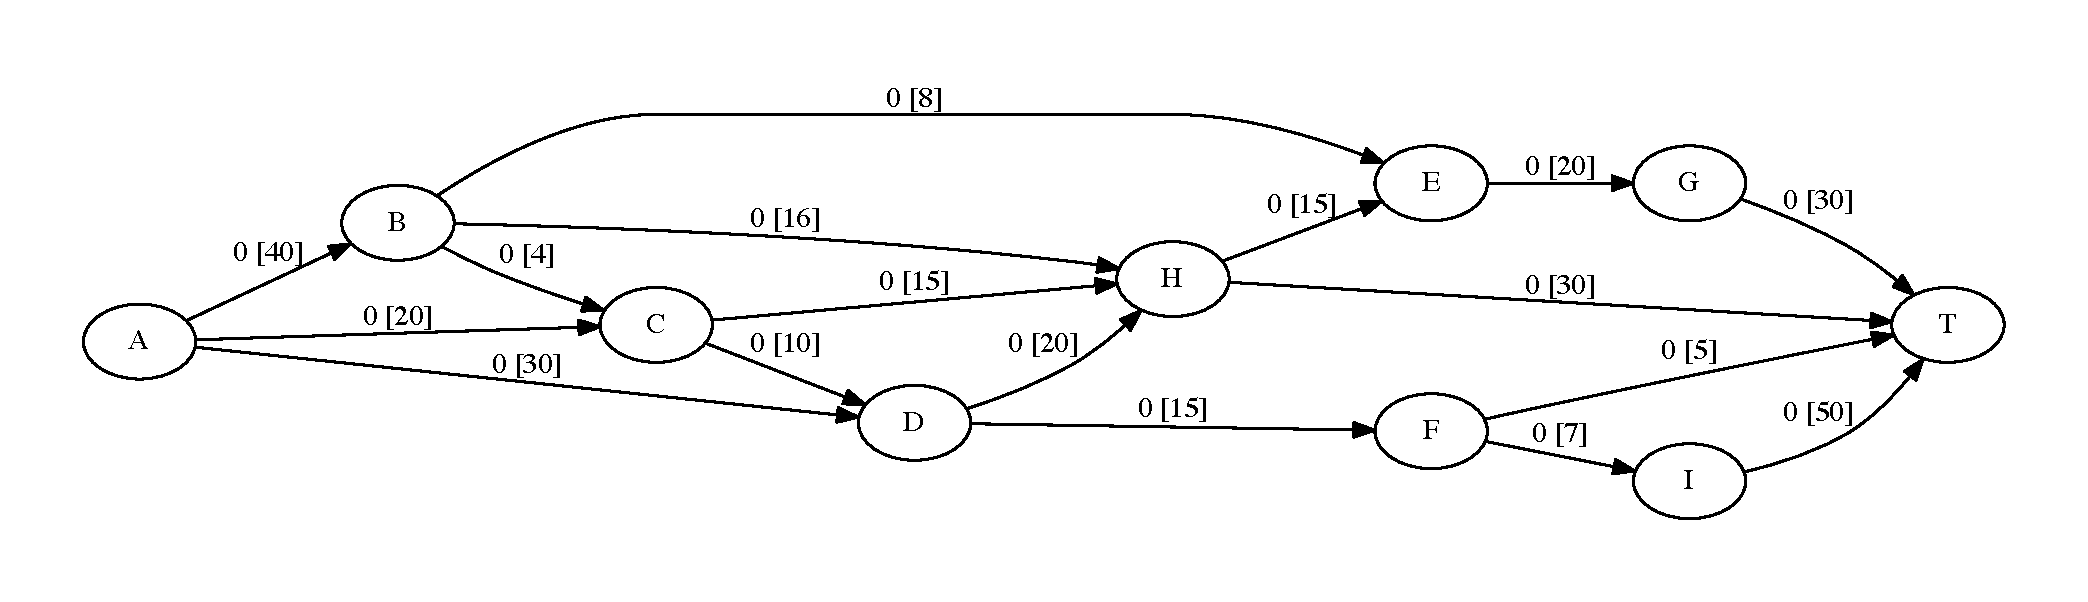
\includegraphics[width=\textwidth]{tutorials/pcc/figs/reseau.pdf}
        \end{center}
        
        
\end{frame}

\begin{frame}{}
    On choisit une première chaîne augmentante : A-B-H-T, on peut augmenter le flot du minimum des capacités, soit 16.
    \begin{center}
        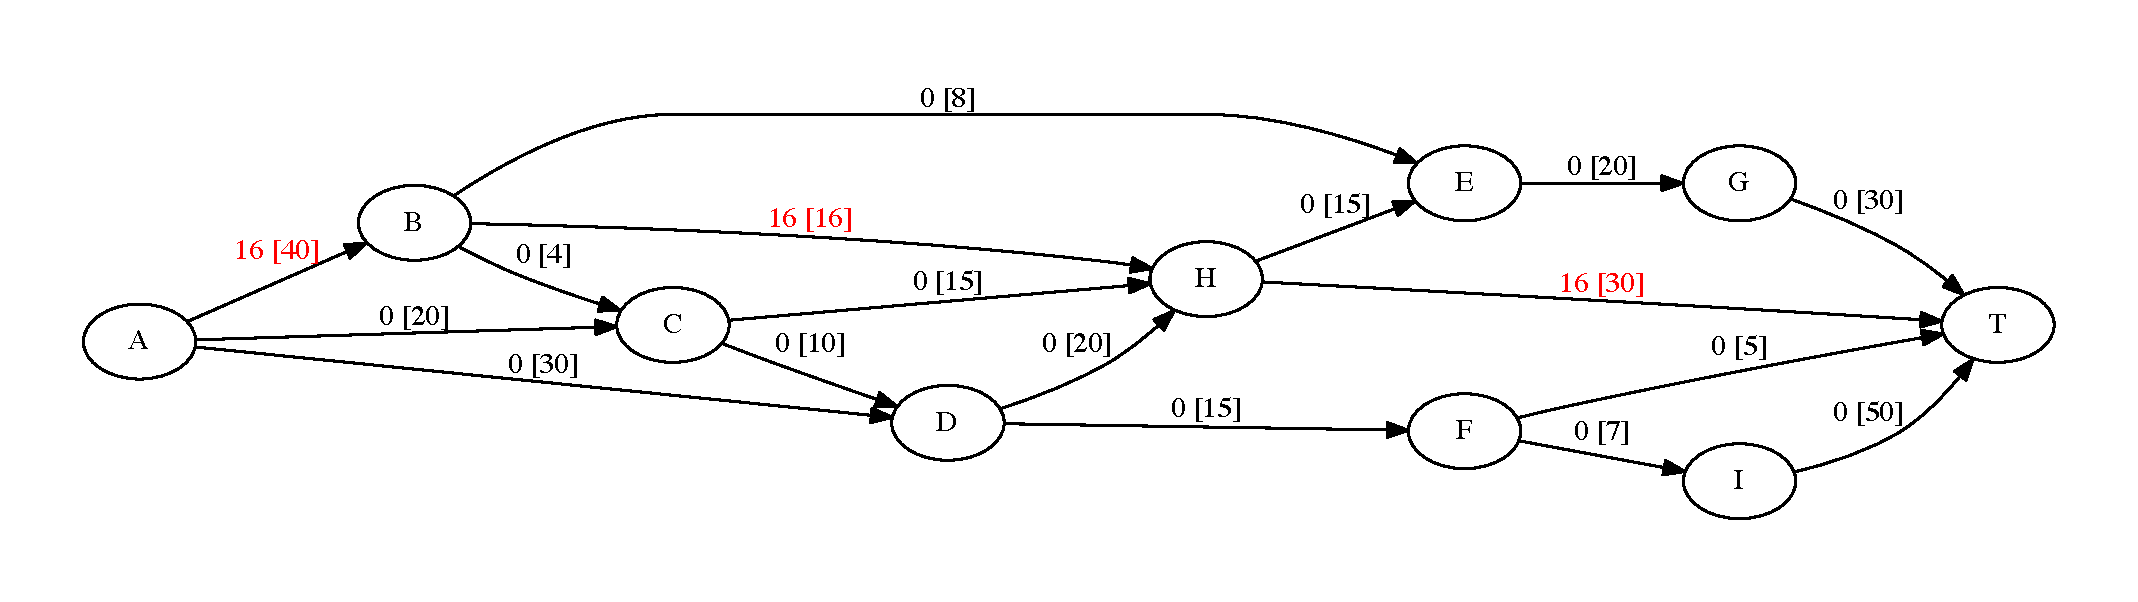
\includegraphics[width=\textwidth]{tutorials/pcc/figs/reseau-1.pdf}
    \end{center}
\end{frame}

\begin{frame}{}
    On choisit ensuite une seconde chaîne augmentante, A-D-F-I-T qui permet d'augmenter le flot de 7.    
    \begin{center}
        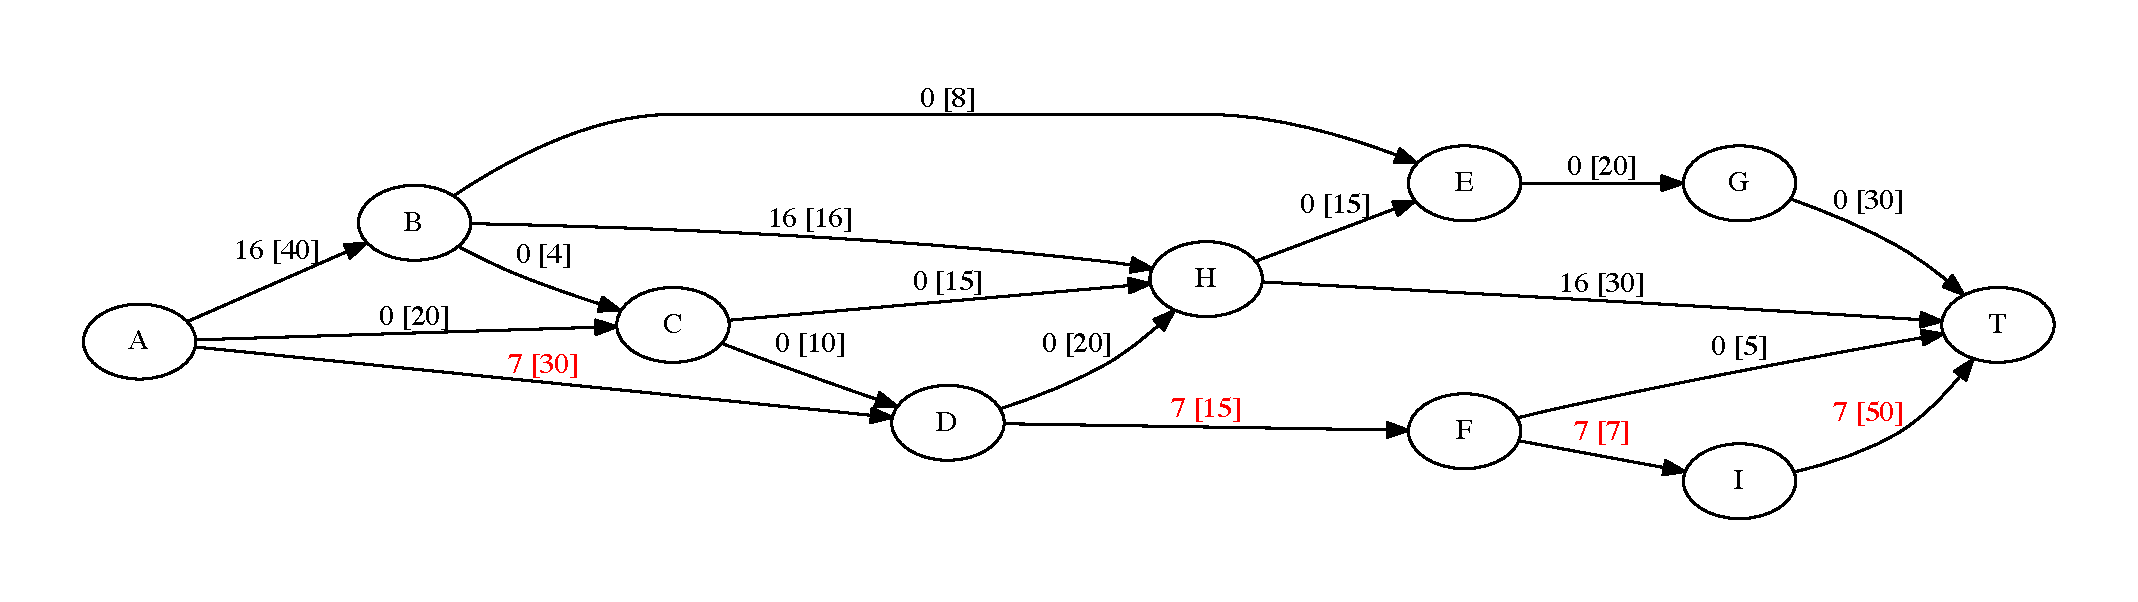
\includegraphics[width=\textwidth]{tutorials/pcc/figs/reseau-2.pdf}
    \end{center}
   
\end{frame}

\begin{frame}{}
    Troisième chaîne augmentante : A-B-E-G-T qui permet d'augmenter le flot de 8. 
    \begin{center}
        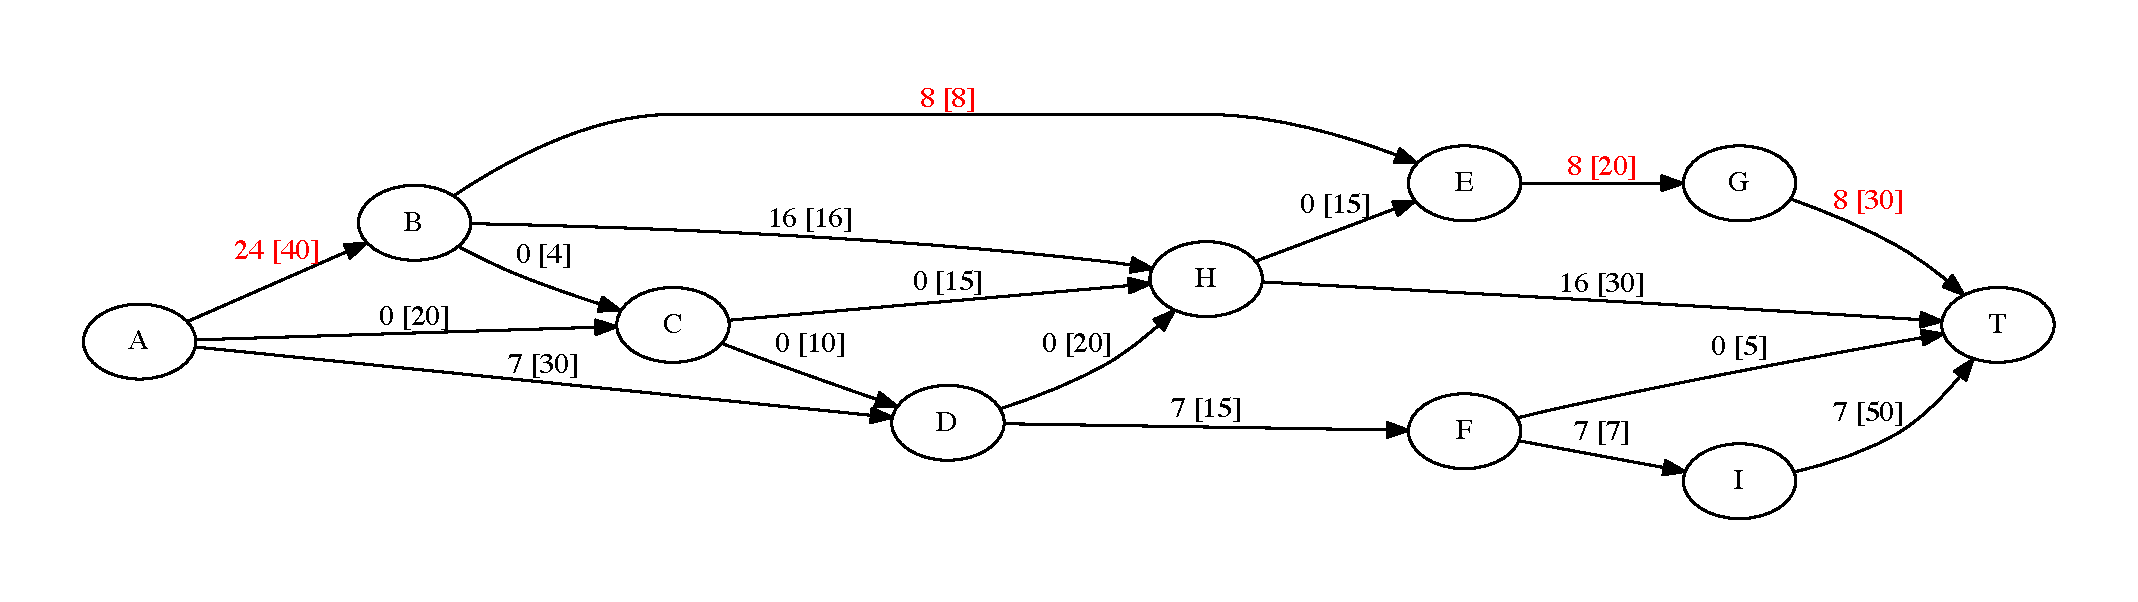
\includegraphics[width=\textwidth]{tutorials/pcc/figs/reseau-3.pdf}
    \end{center}
   
\end{frame}

\begin{frame}{}
    Quatrième chaîne augmentante : A-C-H-T qui permet d'augmenter le flot de 14.
    \begin{center}
        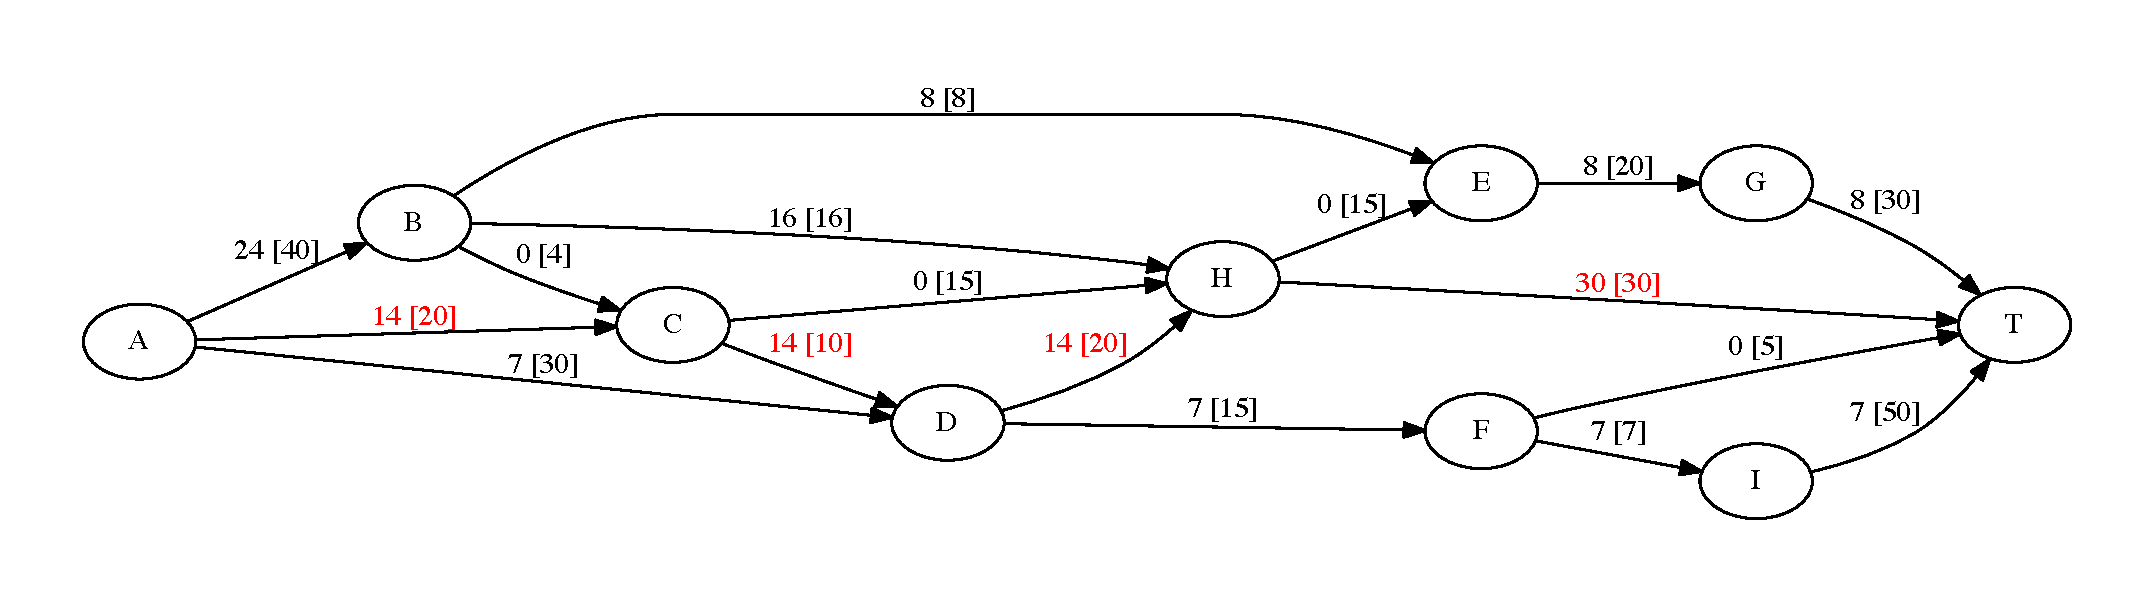
\includegraphics[width=\textwidth]{tutorials/pcc/figs/reseau-4.pdf}
    \end{center}
   
\end{frame}

\begin{frame}{}
    Le graphe devenant moins intuitif, on va appliquer l'algo de marquage.
    \begin{center}
        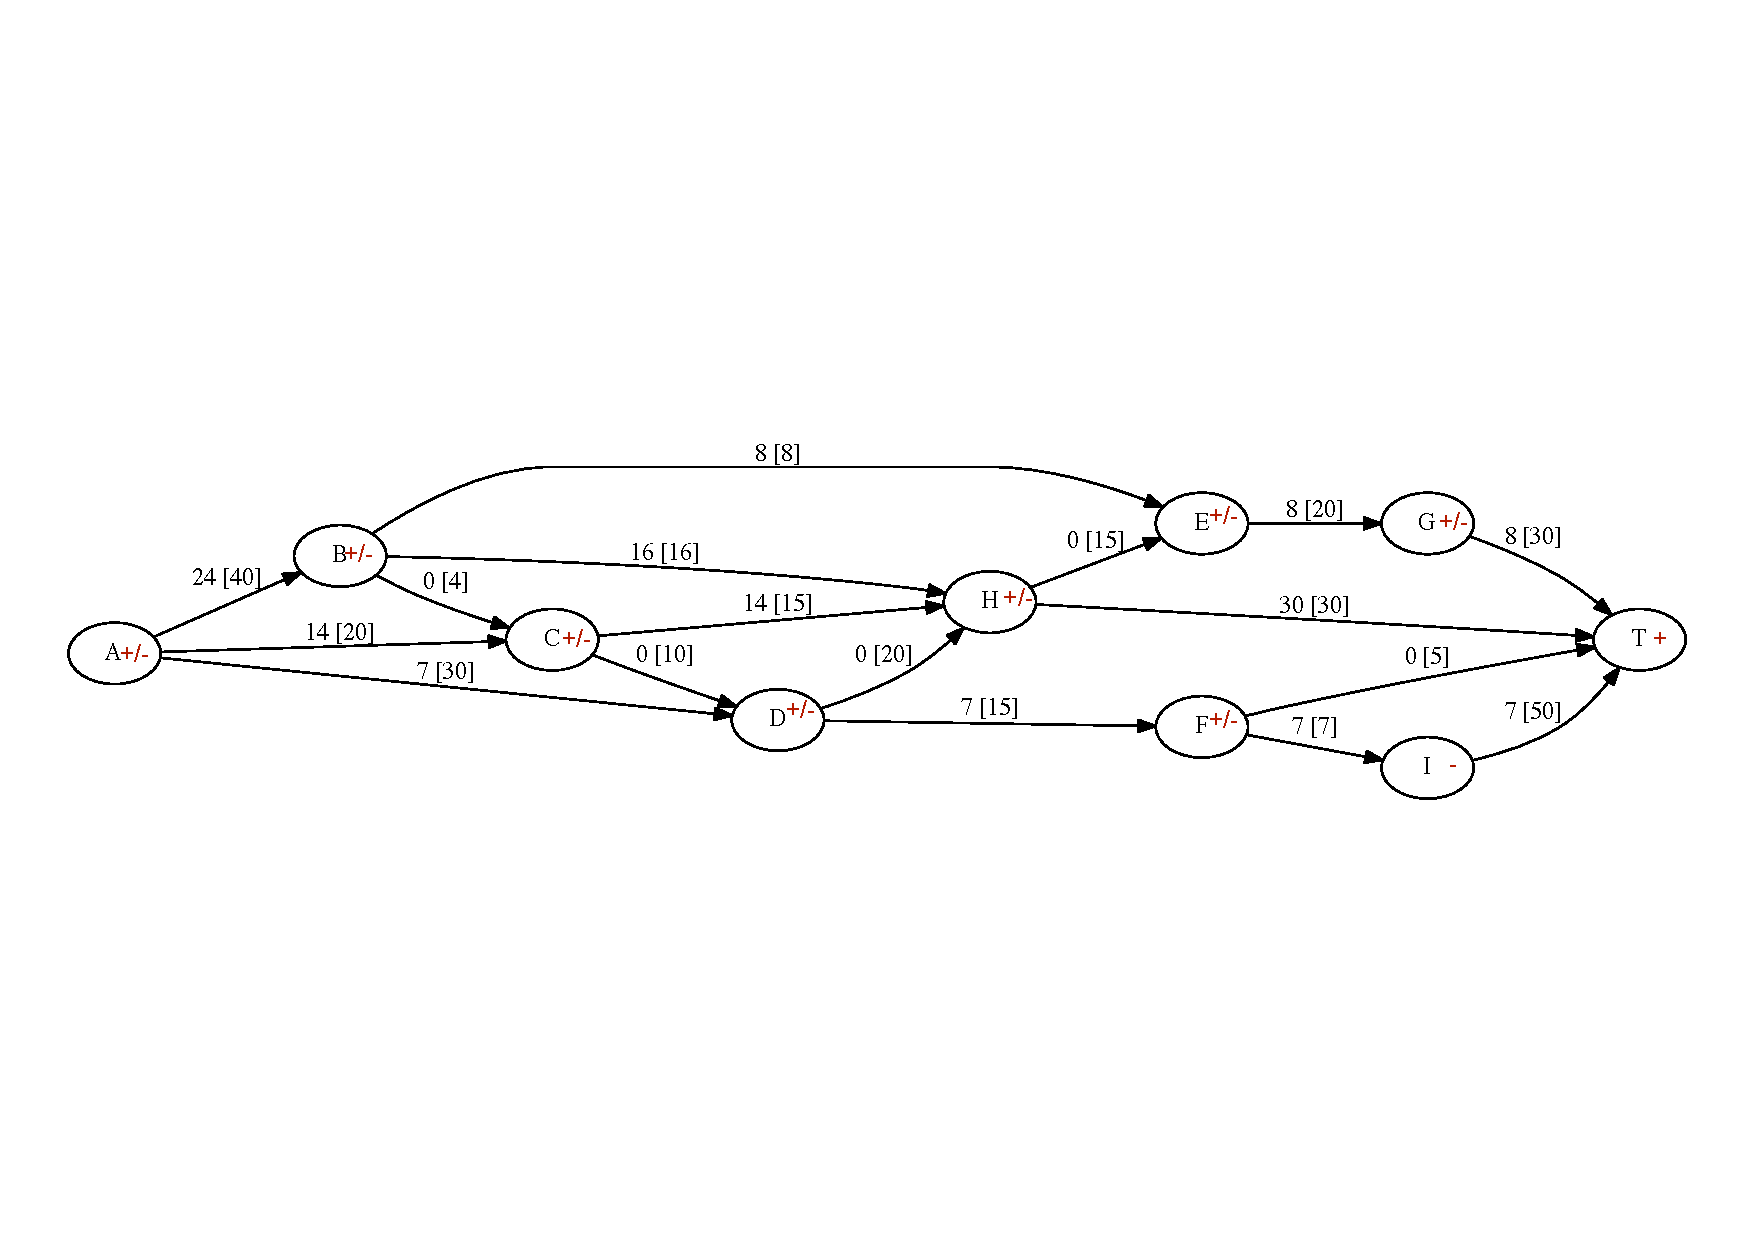
\includegraphics[width=\textwidth]{tutorials/pcc/figs/reseau-4m.pdf}
    \end{center}
   
\end{frame}

\begin{frame}{}
    Ce marquage permet de trouver une chaîne augmentante : A-D-H-E-G-T qui nous permet d'augmenter le flot de 12.
    \begin{center}
        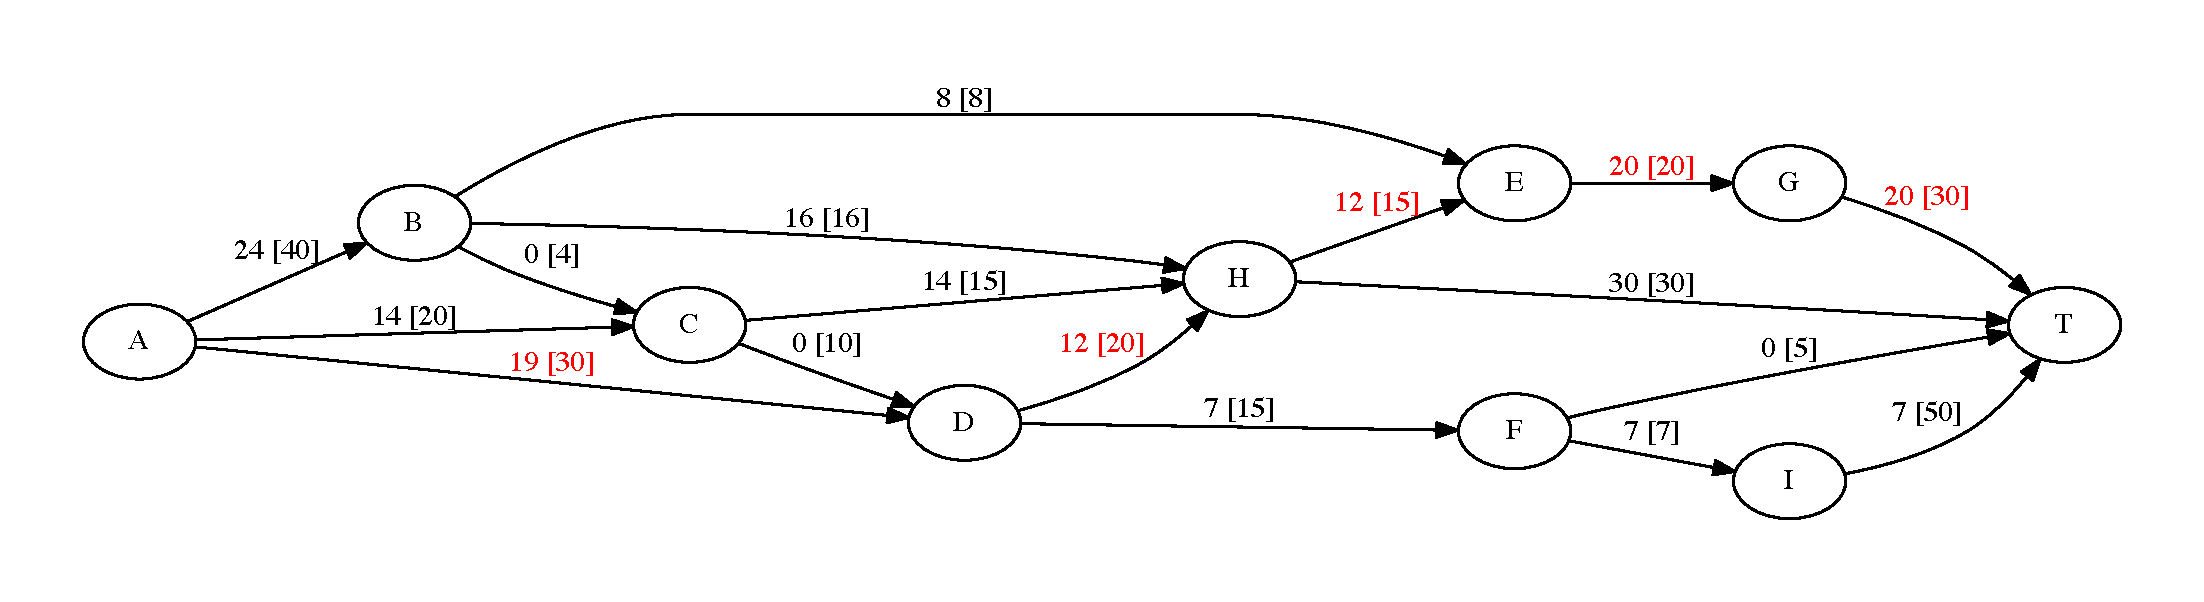
\includegraphics[width=\textwidth]{tutorials/pcc/figs/reseau-5.pdf}
    \end{center}
   
\end{frame}

\begin{frame}{}
    On recommence l'algorithme de marquage.
    \begin{center}
        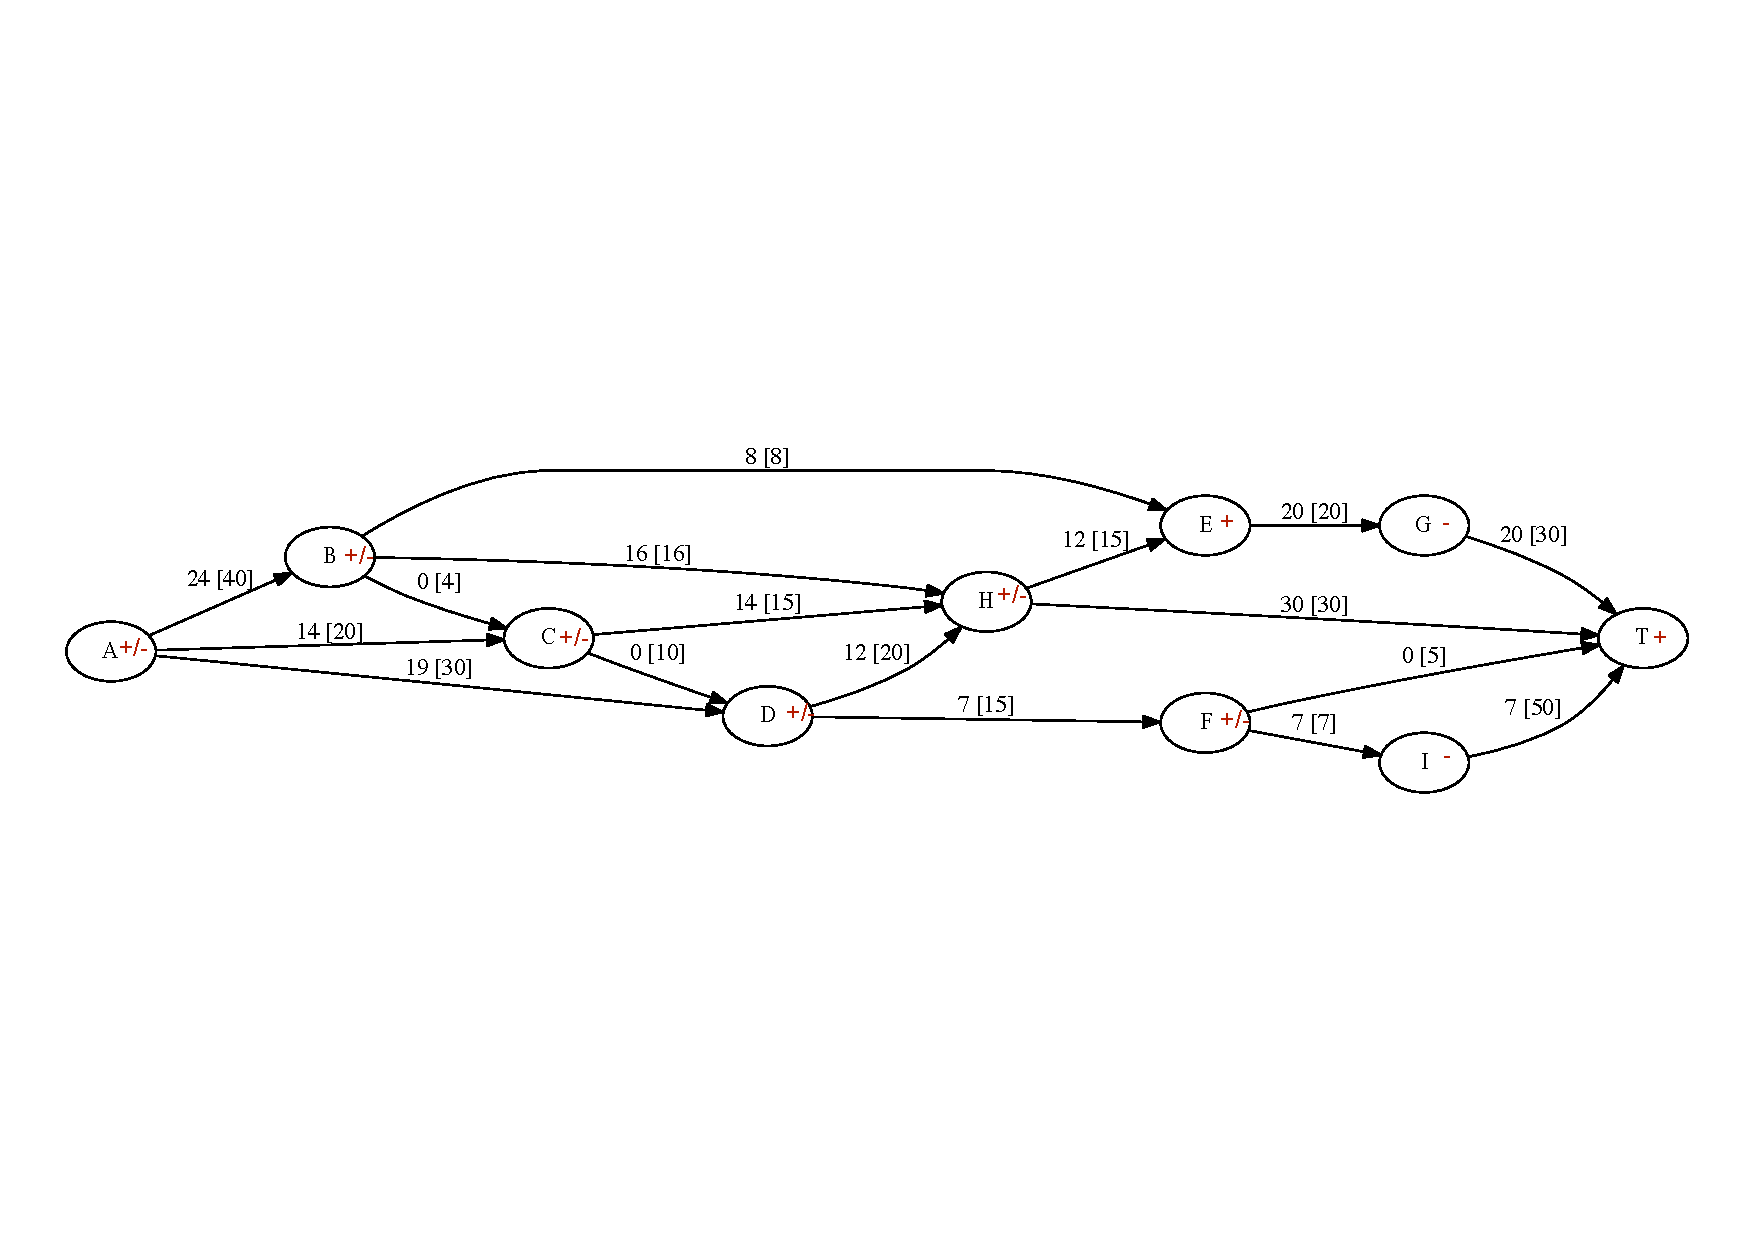
\includegraphics[width=\textwidth]{tutorials/pcc/figs/reseau-5m.pdf}
    \end{center}
   
\end{frame}

\begin{frame}{}
    Celui-ci nous donne une chaîne augmentante A-C-D-F-T qui permet d'augmenter le flot de 5.
    \begin{center}
        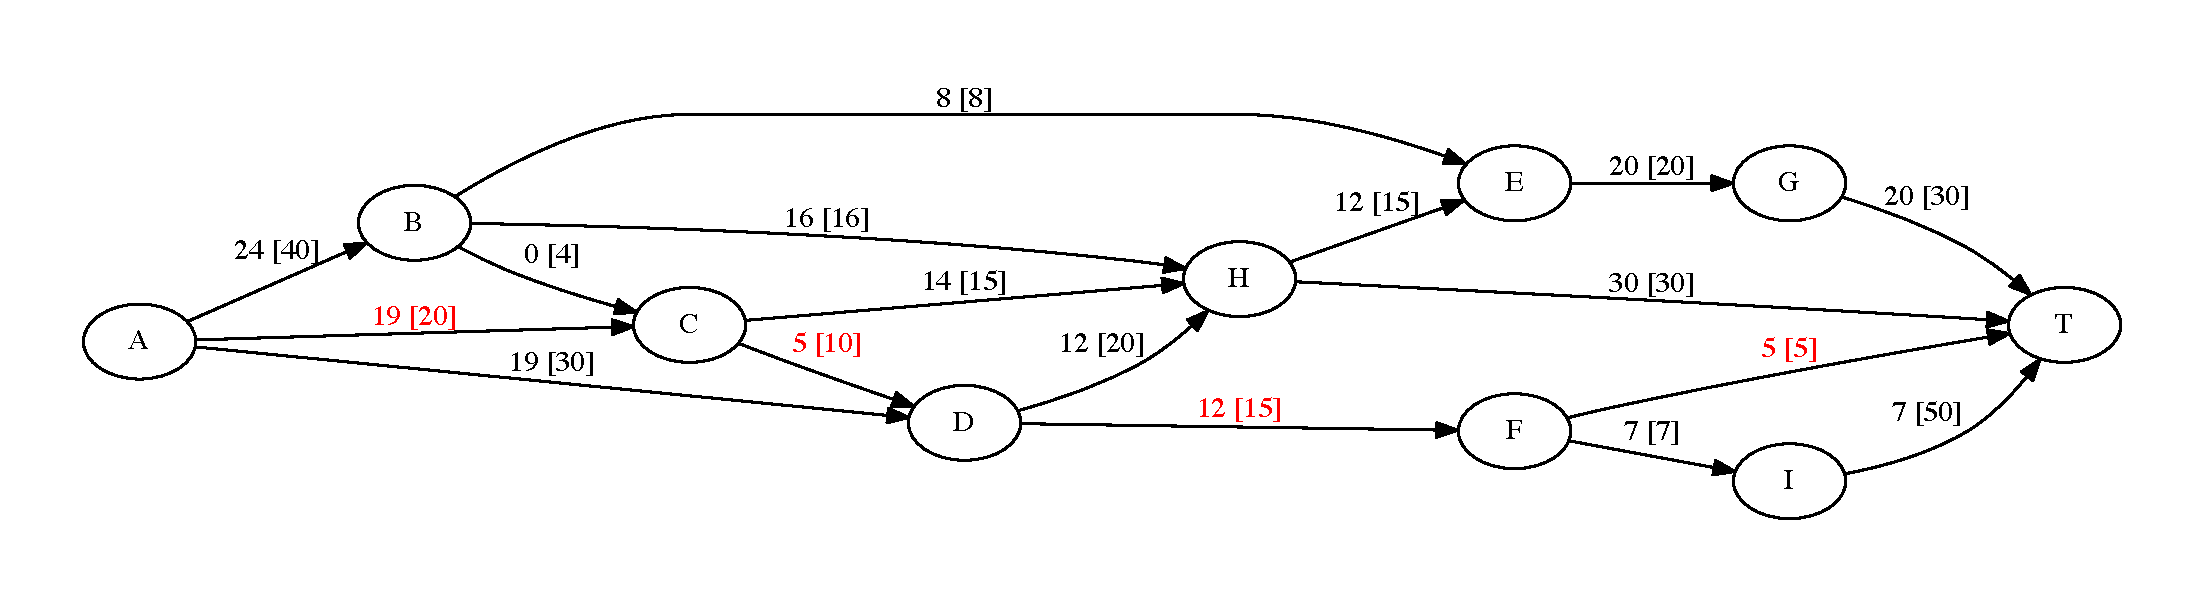
\includegraphics[width=\textwidth]{tutorials/pcc/figs/reseau-6.pdf}
    \end{center}
   
\end{frame}

\begin{frame}{}
    On ré-applique l'algorithme de marquage. Le sommet $T$ n'étant pas marqué +, l'algorithme est terminé. On vérifie en traçant la coupe, la capacité de celle-ci est de 62.

    \begin{center}
        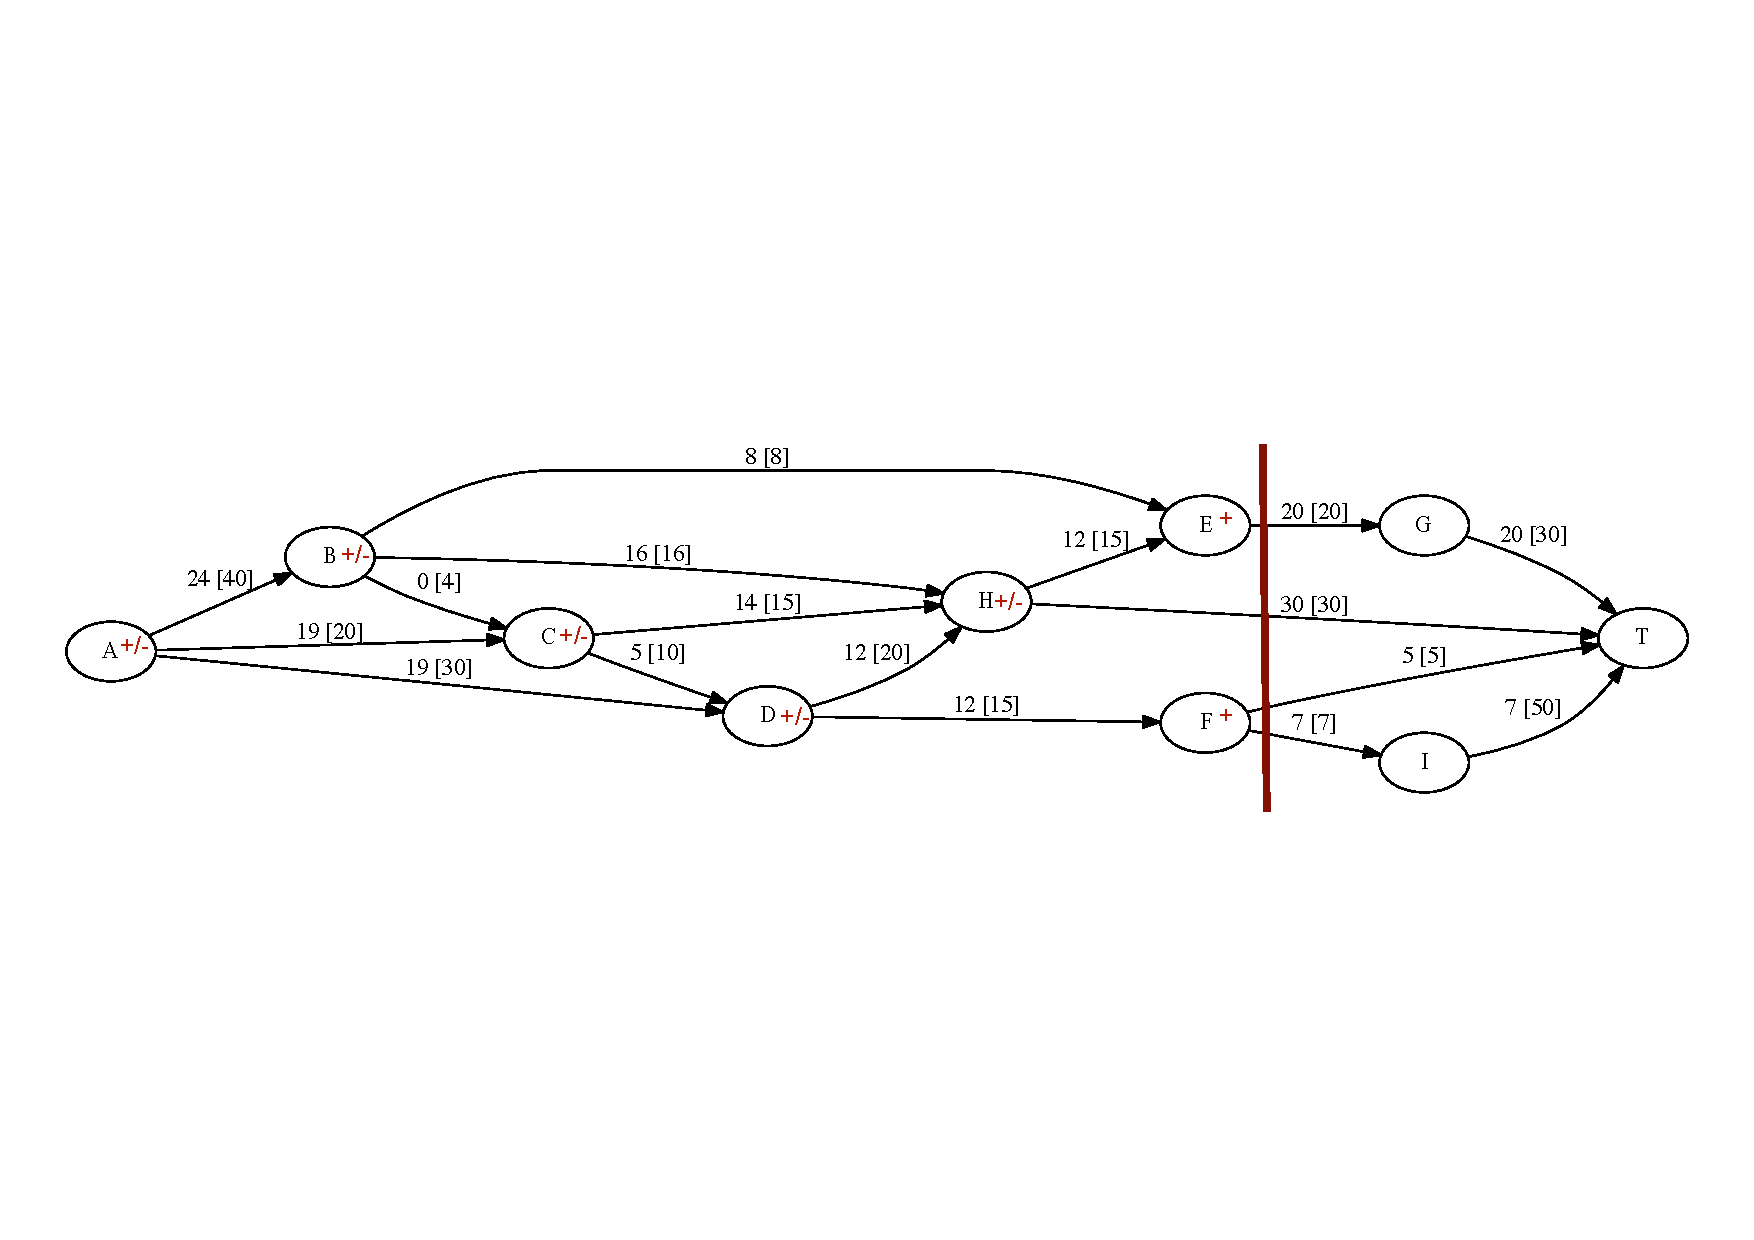
\includegraphics[width=\textwidth]{tutorials/pcc/figs/reseau-6m.pdf}
    \end{center}
   
\end{frame}
